\chapter{Asking Millionaires What They Are Investing In}

We begin not with a theorem but with a repeated question. The School of Hard Knocks host goes into downtown Austin and asks what people are actually investing in, and the answers gradually assemble a practical map of wealth: some answers are about portfolios, some about spending, some about character, and some about timing. These companion notes follow that sequence closely and are curated for this volume by LazyingArt LLC. Where the lecture gives us only a verbal mechanism, we write the minimum mathematics needed to keep the argument sharp without pretending that the source itself is a blackboard derivation.

\section{Opening Survey}

The lecture opens by fixing the asset universe. Before any interviewee tells us what to buy or avoid, the host frames the search broadly: stocks, real estate, and cryptocurrency. That opening move matters, because it tells us that the lecture is not yet choosing a doctrine; it is defining the space in which later judgments will live.

\begin{equation}
\mathcal{A}
=
\{\text{Cryptocurrency},\ \text{Real Estate},\ \text{Stocks/Public Markets}\}.
\end{equation}

We should read this not as a complete taxonomy of wealth, but as the visible starting point of the survey. The lecture begins in the language of categories before it moves into the language of mechanism.

\begin{figure}[htbp]
\centering

\includegraphics[width=0.86\textwidth]{lecture_139_figure_02.png}
\caption{Opening montage of crypto, real estate, and public-market investing.}
\end{figure}

The screenshot remains useful because it shows how the video itself organizes the question. The floating chart fragments in the lower panel, including values such as \(3.15\%\) and \(325\), are not reliable lecture data; they belong to generic market imagery. What survives cleanly is the three-part layout.

\begin{figure}[htbp]
\centering
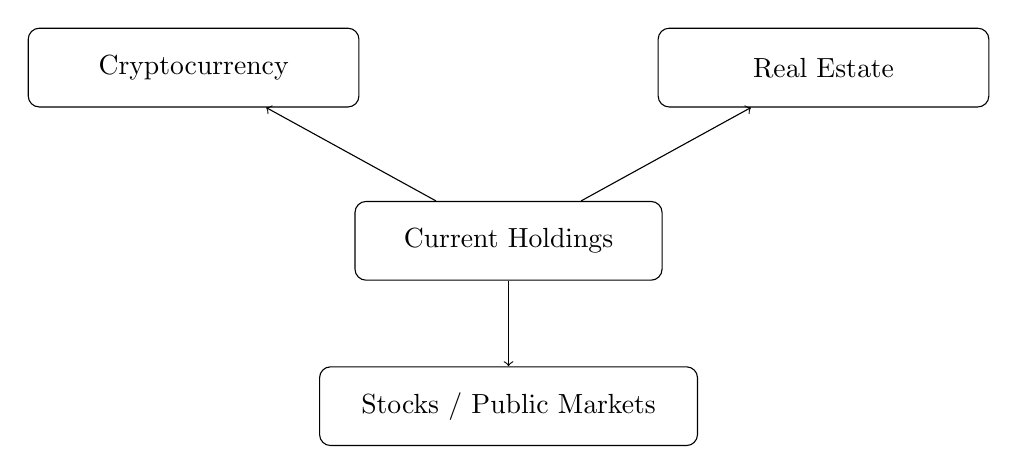
\begin{tikzpicture}
\node[draw, rounded corners, minimum width=3.9cm, minimum height=1cm] (center) at (0,0) {Current Holdings};
\node[draw, rounded corners, minimum width=4.2cm, minimum height=1cm] (crypto) at (-4,2.2) {Cryptocurrency};
\node[draw, rounded corners, minimum width=4.2cm, minimum height=1cm] (realestate) at (4,2.2) {Real Estate};
\node[draw, rounded corners, minimum width=4.8cm, minimum height=1cm] (stocks) at (0,-2.1) {Stocks / Public Markets};
\draw[->] (center) -- (crypto);
\draw[->] (center) -- (realestate);
\draw[->] (center) -- (stocks);
\end{tikzpicture}
\caption{A cleaned conceptual reading of the opening asset map.}
\end{figure}

The redrawn diagram is deliberately simpler than the screenshot. It keeps the structural fact that the lecture opens with three buckets, without pretending that the visual stock chart below is a usable quantitative object.

\section{Skepticism, Dividend Stocks, and Compounding}

The first interviewee does something subtle. He does not begin with a ticker or an allocation rule. He begins with distrust of inherited scripts. One should not simply believe what one is told; one should figure things out, because algorithmic decision systems have weakened the old promise that if we do \(x\), then we reliably get \(y\). The lecture therefore moves from social diagnosis to portfolio behavior: if the environment is less legible, one response is not maximal aggression but defensive consistency.

\paragraph{Anecdote.}
The older path of good behavior, modest conformity, and gradual promotion is explicitly contrasted with the present. Even the mention of the Peter Principle comes in as part of a story about a career ladder that no longer behaves predictably.

\paragraph{Claim.}
The portfolio answer is conservative high-dividend stocks: they do not win as much in exuberant markets, but they also do not lose as much when conditions deteriorate.

\paragraph{Mechanism.}
We can encode that verbal asymmetry in a compact way:
\begin{align}
R_{\text{good}}^{\text{div}} &< R_{\text{good}}^{\text{mkt}}, \\
\left|R_{\text{bad}}^{\text{div}}\right| &< \left|R_{\text{bad}}^{\text{mkt}}\right|.
\end{align}
This is not an empirical estimate from the video. It is the clean mathematical form of the interviewee's point: smaller upside in the boom, smaller damage in the slump.

\subsection{Question \& Answer}

The lecture now raises its first real technical question: how can someone become financially free in 2022? The answer is deliberately anti-magical. Compounding is your friend, and therefore one year is usually too short a horizon.

To make that statement precise, we introduce a discrete wealth update rule. Let \(W_n\) be wealth after \(n\) periods, let \(r\) be the effective periodic return, and let \(C_{n+1}\) be the contribution made at the next step. Then
\begin{equation}
W_{n+1} = (1+r)W_n + C_{n+1}.
\end{equation}
This is the natural recursion for a portfolio that both grows and receives fresh savings.

If we iterate that rule, we obtain the closed form
\begin{equation}
W_n = W_0(1+r)^n + \sum_{k=1}^{n} C_k (1+r)^{\,n-k}.
\end{equation}
The derivation is elementary but worth writing once:
\begin{enumerate}
\item Start from \(W_{n+1} = (1+r)W_n + C_{n+1}\).
\item Substitute \(W_n = (1+r)W_{n-1} + C_n\).
\item Continue the substitution until we reach \(W_0\).
\item Collect the powers of \((1+r)\) multiplying each older contribution.
\end{enumerate}
The speaker's practical point now becomes transparent. Unless we begin with unusually large initial capital, unusually large cash flows, or unusually high returns, the exponential benefit of compounding needs time to matter.

For constant contributions \(C_k=C\), we get the familiar special case
\begin{equation}
W_n = W_0(1+r)^n + C\,\frac{(1+r)^n-1}{r}.
\end{equation}
This is enough to justify the lecture's refusal of the one-year fantasy. The question is not merely how to get rich quickly; it is how to choose a mechanism that does not collapse under ordinary time.

\section{Energy, Drawdowns, and Character}

The next interview shifts the tone. The speaker is retired from the military, now in consulting, and currently invested in energy stocks. But the market context matters: he is hunkered down because the market has dropped sharply that day. The lecture moves from asset class to stress condition.

We can summarize the market shock minimally as
\begin{equation}
\Delta I_{\text{day}} < -1000 \ \text{points}.
\end{equation}
Here \(\Delta I_{\text{day}}\) is only a stress marker. The transcript does not identify the precise index, and it would be a mistake to pretend that it does. What matters is the scale of the one-day disturbance.

The answer to that disturbance is not given as a trading algorithm. Instead, the interviewee turns to a triad:
\begin{itemize}
\item intelligence,
\item integrity,
\item initiative.
\end{itemize}
And then, one question later, to discipline and self-discipline.

This is a characteristic move in the lecture. We begin with a portfolio position, but we are immediately told that the deeper problem is the formation of the person who must live through volatility. In these notes, we should preserve that move. The lecture is not content with saying what to hold; it wants to say what sort of person can hold it without dissolving under noise.

\section{Human Sales and Values-Based Freedom}

The next voice comes from media and advertising, specifically from sales at TikTok. The allocation answer is modest and ordinary: a little crypto, the basics in mutual funds, and some other companies. But again the lecture uses the portfolio answer only as an entrance. The real point is the manner in which one moves through economic life.

\paragraph{Anecdote.}
When asked about sales, the speaker says the secret is being human. One cannot sell well by forgetting that the other person goes home to somebody, has a home life, may need to pick up a child, may simply want a drink after work.

\paragraph{Claim.}
The claim is that economic interaction works better when we remember the full human context instead of abstracting the counterparty into a revenue target.

\paragraph{Mechanism.}
This then becomes a second answer to the question of financial freedom. The lecture does not repeat the first answer; it deliberately changes the mechanism. This time the mechanism is values-based spending.

\subsection{Question \& Answer}

How can someone become financially free in 2022? The answer here is not ``maximize every financial instrument.'' It is ``identify what matters and let spending reflect it.''

Let \(E_i\) denote spending on priority \(i\), and define the spending share
\begin{equation}
s_i = \frac{E_i}{\sum_j E_j},
\qquad
\sum_i s_i = 1.
\end{equation}
This is the minimal formalization of the speaker's idea. Financial freedom, in this answer, is not merely the level of resources; it is the alignment between actual expenditure shares and chosen values.

The lecture makes the point concretely, not abstractly. Priority categories include gym, healthy eating, organic food, travel, and whatever else the person genuinely values. The useful distinction is therefore not
\[
\text{frugal} \quad \text{versus} \quad \text{extravagant},
\]
but rather
\[
\text{aligned spending} \quad \text{versus} \quad \text{unexamined spending}.
\]
The first answer used time; the second uses selection. The lecture wants both answers to stand.

\section{Vocation and the Day-Two Reset}

At this point the lecture slows down. Another interviewee says that he would tell his younger self to take things more seriously, but the answer does not collapse into pure regret. It opens into a story about music, DJ work, and then a career through major labels. This matters because the lecture is refusing a single linear model of success. Seriousness matters, but it does not erase vocation.

Then the host explicitly resets the frame: this is day two, they are back out downtown, the earlier day was thin, and they want a broader spread of answers. This reset is not filler. It tells us that the lecture is conscious of sample size. The inquiry is being reopened because the first cluster of voices was not enough.

We should therefore preserve the reset as a structural hinge. The chapter is not a collection of stray quotations; it is a second pass through the same question, now with a widened search.

\section{Self-Investment, Timing, and the Collection Phase}

The late part of the lecture broadens the meaning of investment still further. A surgeon appears, rejects degree worship in stark language, and answers the investment question with real estate, oneself, and other people one trusts. Here the asset universe expands beyond formal securities into self-capital and trusted networks.

A little later, another answer on education becomes more conditional rather than categorical: some people prove that a degree is unnecessary, some prove that it is useful, and the real task is to identify one's own path. This then leads to business advice: follow what you love closely enough that you can ask how to monetize it. In other words, path choice is itself part of the investment problem.

\paragraph{Anecdote.}
The lecture now contains several non-identical notions of investment:
\begin{itemize}
\item real estate,
\item oneself,
\item trusted people,
\item a vocation one would pursue even before monetization.
\end{itemize}

\paragraph{Claim.}
The claim is not that all these objects are interchangeable. The claim is that wealth-building includes judgment about where productive agency actually lives.

\paragraph{Mechanism.}
That broader view prepares the lecture for a sharper question about timing.

\subsection{Question \& Answer}

What do we do in a tricky market? The real-estate developer gives the cleanest late answer. Crypto is described as young, energetic, and volatile; stocks are described as much older and therefore more settled. The maturity analogy can be written as
\begin{equation}
T_{\text{crypto}} \approx 10\text{--}15 \ \text{years},
\qquad
T_{\text{stocks}} \approx 100 \ \text{years}.
\end{equation}
This is not a theorem, only a disciplined analogy. Age stands in for maturity; maturity stands in for lower volatility.

The real estate advice is even more interesting. Interest rates are rising, the environment is uncertain, and therefore the best trade may be not to trade. We can write that local decision rule as
\begin{equation}
V_{\text{wait}} > V_{\text{buy-now}}
\end{equation}
for the particular market state being described. Again, this is not universal. It is the mathematical shadow of the spoken recommendation: under current conditions, sitting on the sidelines may dominate immediate entry.

The lecture closes this arc by moving from investing to collecting. A retired dentist says he is done investing and now collecting, then names equities, annuities, bonds, and the yearly cash flows they produce. The phase shift can be written as
\begin{equation}
CF_{\text{year}} = CF_{\text{eq}} + CF_{\text{ann}} + CF_{\text{bond}}.
\end{equation}
This formula does very little formally, but that is precisely its virtue here. It marks the change in objective. We are no longer maximizing future optionality; we are summing present income streams.

The speaker's advice about advisors is equally concrete: many advisors were useless, and one finally worked. The lecture ends, then, not with a grand abstract law, but with a recognizably adult sequence of tasks:
\begin{itemize}
\item build,
\item wait when waiting is better,
\item collect when the collection phase begins,
\item keep searching for competent help.
\end{itemize}

\section{Summary}

The lecture begins with a public survey and ends with a life-cycle picture of wealth. Along the way we are given several distinct mechanisms: defensive dividend exposure, the long arithmetic of compounding, the role of character under drawdown, values-based spending, self-investment, the option value of waiting, and finally the transition from accumulation to collection.

What makes the sequence worth preserving is that it does not collapse these mechanisms into one slogan. The same question --- what are you investing in, and how do you become free? --- is answered by different people from different stages of life. The resulting chapter should therefore keep the multiplicity. We do not leave with a single formula for wealth. We leave with a small bank of mechanisms, each introduced where the lecture itself found the need for it.